\begin{frame}
\frametitle{Additional simulation and analysis}       
\begin{textblock*}{12.5cm}(0.1cm,2.2cm) % {block width} (coords)
	\begin{figure}[ht!] % replace 't' with 'b' to force it to 
		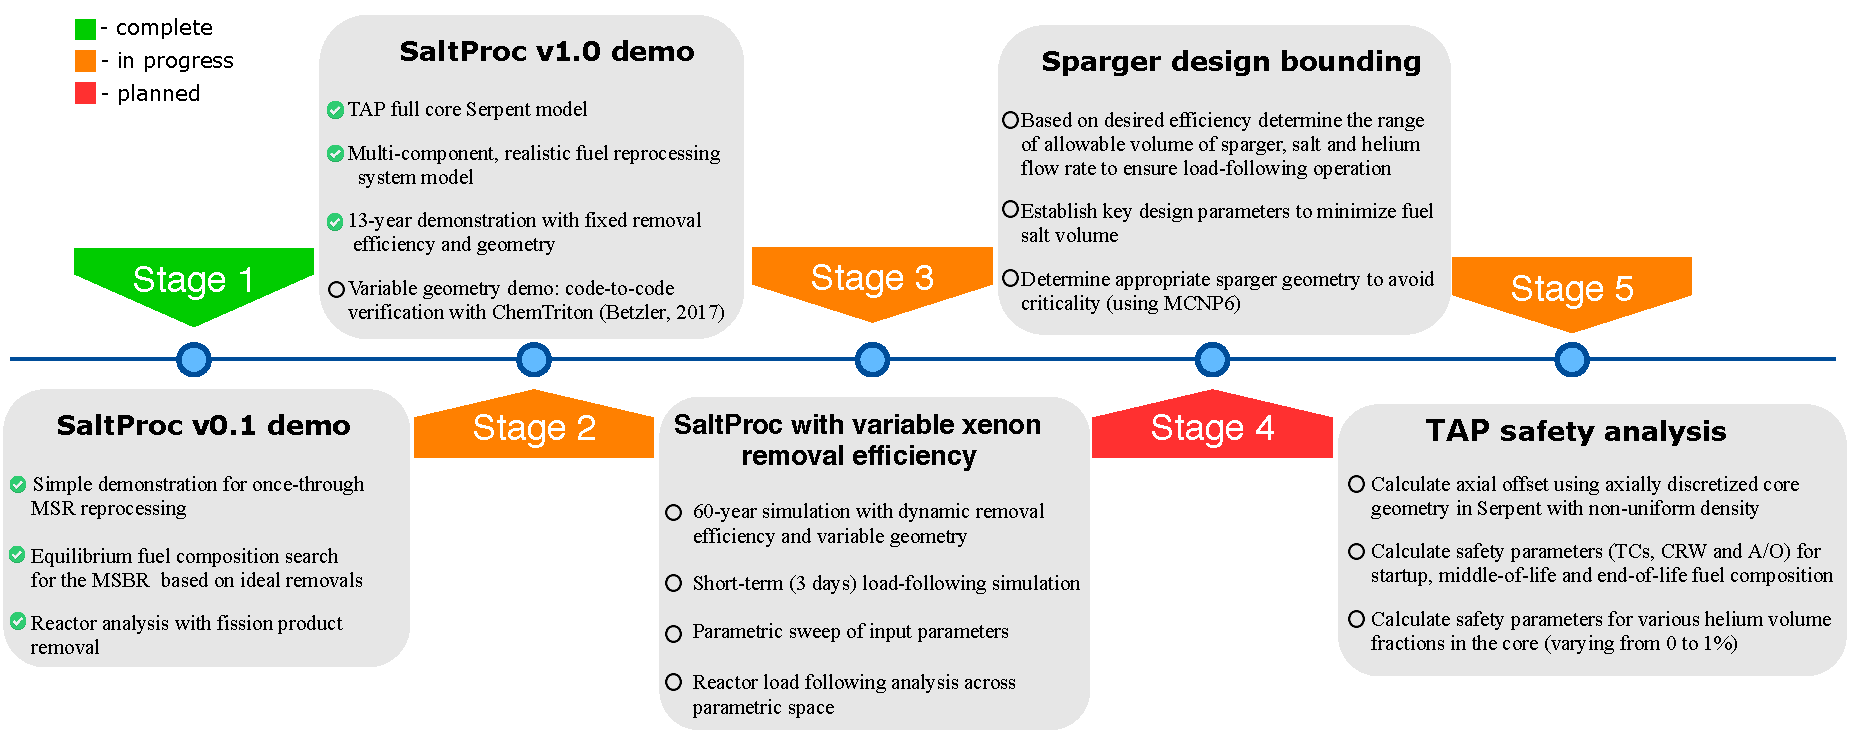
\includegraphics[width=\textwidth]{./images/progress_chart.pdf} 
	\end{figure}
\end{textblock*}
\end{frame}


\begin{frame}
\frametitle{SaltProc demonstration for realistic on-line reprocessing system}
	\begin{block}{Finishing Stage 2}
		\begin{enumerate}
			\item Implement variable core geometry capability in SaltProc
			\item Demonstrate a key feature of
the \gls{TAP} reactor - 
			adjusting the moderator rod configuration - which is necessary 
			achieve 60-years lifetime.
			\item Perform 40-year depletion simulation using SaltProc 
			and compare obtained results with Betzler \emph{et al.} 
			\cite{betzler_assessment_2017}
		\end{enumerate}
	\end{block}
	
	\begin{block}{Stage 3: SaltProc demonstration with variable Xe removal 
	efficiency}
		\begin{enumerate}
			\item Incorporate extraction efficiencies as a function of many 
			physical system design
parameters (e.g., void fraction in the 
			salt, helium bubble size)
			\item Perform life-time long depletion simulation with dynamic 
			removal efficiency
			\item Perform short-term (3 days) depletion with the core power 
			changing in the [0, 100\%] range with a ramp rate 10\%/min
			\item Conduct parametric sweep of input parameters in the xenon 
			extraction equation to determine the range of key parameters when 
			load-following is possible
		\end{enumerate}
	\end{block}
\end{frame}


\begin{frame}
\frametitle{Gas removal system bounding and safety analysis for the TAP}
\begin{block}{Stage 3: Prototype design for the Xe removal system}
	\begin{enumerate}
		\item Determine bounds for key design parameters (sparger volume, 
		geometry, salt and helium flow rates) by analyzing parametric sweep
		\item Calculate key design parameters to minimize fuel salt inventory 
		in the system
		\item Perform nuclear criticality safety analysis using MCNP6 
		\cite{werner_mcnp6._2018} to
confirm that the selected 
		sparger design is safe
	\end{enumerate}
\end{block}

\begin{block}{Stage 5: \gls{TAP} Safety and Operational parameters analysis}
	\begin{enumerate}
		\item Finish a axially discretized core
geometry in Serpent with 
		non-uniform axial density distribution to estimate the axial power
		offset
		\item Calculate safety parameters (temperature coefficients, control 
		rod worth, axial power offset) at the \gls{BOL}, the middle-of-life, 
		and the \gls{EOL}
		\item Repeat for short-term depletion to capture the parameters 
		dynamics for load-following operation
	\end{enumerate}
\end{block}
\end{frame}


\begin{frame}
\frametitle{Conclusion}
	\begin{textblock*}{12cm}(0.4cm,2cm) % {block width} (coords)
	\begin{itemize}
		\item Motivation for the developing fuel processing simulation tool 
		for liquid-fueled nuclear reactors have been outlined
		\begin{itemize}
			\item Fuel salt processing systems modeling in \glspl{MSR} have 
			historically been conceptual rather than concrete
			\item This work will more realistically model salt processing 
			system with a focus
on the gas removal system of the prospective 
			\gls{TAP} \gls{MSR}
		\end{itemize} 
		\item Preliminary results obtained using SaltProc include:
			\begin{itemize}
				\item Simple demonstration for \gls{MSBR} with ideal/fixed 
				fission products removal efficiency
				\item Multi-component fuel reprocessing system modeling 
				for \gls{TAP} with non-ideal/constant efficiency
				\item Determining the effect of fission product removal on the 
				core neutronics
			\end{itemize}
		
		\item Future work
			\begin{itemize}
				\item Add variable geometry and dynamic removal efficiency 
				capability to realistically model the \gls{TAP} system
				\item Demonstrate and validate those capabilities for 
				lifetime-long depletion simulations
				\item Simulate the \gls{TAP} reactor behavior in short-term 
				transients to determine the
feasibility of load following
				\item Determine feasible design parameters of the sparger, 
				critical component of the
TAP gas removal system
				\item Analyze dynamics of the safety parameters for long-term 
				and short-term cases
			\end{itemize}
	\end{itemize}
\end{textblock*}
\end{frame}
